

\begin{frame}{\ft{Room-By-Room Tab Organization}}

\doubleFrame{The Room-by-Room breakdown features a dual tabbed 
area: on the top appear the room tabs, and to the left appear 
the feature tabs.  The combination of 
currently selected room and feature tabs 
control the highlighting of details in room descriptions.  
Realtors will have the flexibility to choose which features 
to describe and which rooms to include in the breakdown.}

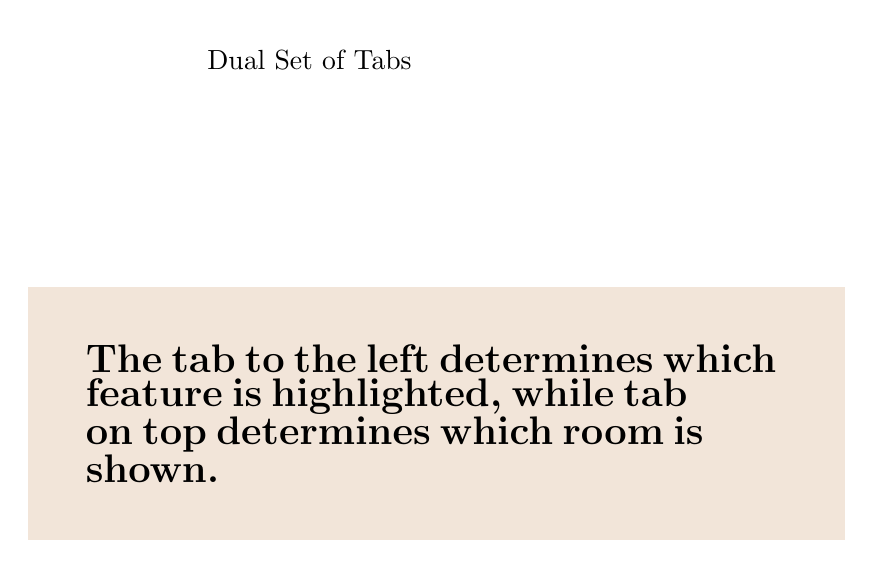
\begin{tikzpicture}
\nodeincludegraphicsTR{5.5cm}{3cm}{screenshots/ss-rm2.png}

\node [anchor=west,fill=white,inner sep=8]
 (note) at (10,8) {\hc{Dual Set of Tabs}};

\ann{darkRed}{0.7}{1mm}{grammarArrowColor}{0.5}{12,10.5}{6.5}{1}{0.85}

\colorarr{>=latex, ->}{fcBoxColor!20!black}
{0.8}{blGreen!30!red}{2}{1mm}{note.north}{15, 10}

\colorarr{>=latex, ->}{fcBoxColor!20!black}
{0.8}{blGreen!30!red}{1}{1mm}{note.west}{5.3, 6.2}

 \node [anchor=west,fill=brown!20!white,inner sep=21, text width=8.9cm]
  (longnote) at (8,3.5) {%  %{\color{rb!85!red}{
  {\cframedbox{\Large \textbf{The tab to the left determines which \makebox{feature} is  
highlighted, while tab on top \makebox{determines} which room is shown.}}}};

\ann{BlueGreen}{0.3}{1mm}{grammarArrowColor}{0.5}{3,6}{3}{4.5}{0.95}

\end{tikzpicture}


\end{frame}

